\documentclass[tcc]{ic}

\hypersetup{
    colorlinks = {true},
    linktocpage = {false},
    plainpages = {false},
    linkcolor = {Blue},
    citecolor = {Blue},
    urlcolor = {Red},
    unicode = {true},
    pdftitle = {Alexis Rapport d'apprentissage en entreprise ADITU du 25-12-2023 au 19-01-2024}, 
    pdfauthor = {Alexis Déhu},
    pdfsubject = {Rapport de mes activités chez ADITU pour la période du 25-12-2023 au 19-01-2024},
    pdfkeywords = {activités, alternance, iut, but, rt, aditu, uppa, pau, bidart}
}

\usepackage{algorithm}
\usepackage{algpseudocode}

\makeatletter
\renewcommand{\ALG@name}{Algoritmo}
\renewcommand{\listalgorithmname}{List of \ALG@name s}
\makeatother

\newcolumntype{Y}{>{\centering\arraybackslash}X}

\begin{document}

    % Inclui o preâmbulo do documento (Informações da capa e contracapa)
    \titulo{Rapport d'activités en entreprise}

\autor{Alexis Déhu}{a.dehu@aditu.fr}{}


\orientador{M. Éric Pierre-Sala}{e.pierre-sala@aditu.fr}{}{}{}
\examinador{M. Guillaume Devesa}{g.devesa@aditu.fr}{}{}{}

\dataMesAno{Septembre}{2023}{}

    \selectlanguage{english}
    
    % Capa, contracapa e avaliadores
    \capa

    % \aprovacao
    
    % Agradecimentos
    % \begin{agradecimentos}

Obrigado

\end{agradecimentos}
    
    % Resumo e Abstract
    \begin{resumo}

    Cette deuxième période la plus longue d'enseignements à l'IUT (5 semaines) nous a permis d'aborder un vaste champ de compétences extrêmement utiles et intéressantes selon moi.
    \\ \\
    Nous avons couvert trois modules de notre parcours cybersécurité orienté vers la sécurisation du service DNS avec DNSsec, de la compréhension des attaques utilisées sur des protocoles répandus dans les réseaux locaux d'entreprises et de la compréhension des technologies et pratiques de chiffrement de nos données.
    \\
    Nous avons aussi aussi à manipuler et intégrer des pare-feux physiques dans un réseau local d'entreprise selon leur besoins.
    \\ \\
    Aspect télécommunications, nous avons abordés les réseaux cellulaires 2G, 3G, 4G et d'autres en profondeur, en parallèle avec l'étude physique et mathématique de moyens transmissions modernes d'émission-réception.
    \\ \\
    Un module intéressant était aussi consacré à l'automatisation de nos tâches d'administrations des systèmes et des réseaux. En complément de l'apprentissage d'un anglais professionnalisé et d'un travail sur notre communication.
    
    \palavrasChave{sécurisation; protocoles; ARP; ICMP; DNS; chiffrement; cryptographie; clés; chiffrement symétrique; chiffrement asymétrique; intégrité des données; confidentialité; authentification; authenticité; signature; certificat; fonctions mathématiques et algorithmiques; OFDM; COFDM; MIMO; CDMA; TDMA; FHSS; féseaux cellulaire; filtres numériques; filtres analogiques}
\end{resumo}
    %% \begin{abstract}
%     Lorem ipsum dolor sit amet, consectetur adipiscing elit. Duis elit tellus, vehicula in justo eget, fermentum aliquet nisi. In id quam mauris. Sed id vehicula libero. Quisque id tortor placerat, consequat ex sed, placerat ante. Ut dui nunc, placerat volutpat ipsum sit amet, dictum pellentesque lacus. Donec leo sem, dictum quis lacus at, ultricies sagittis elit. Mauris sit amet tortor efficitur, luctus justo sit amet, tincidunt tellus. Donec vulputate non risus at tincidunt. Sed accumsan at erat in aliquet. Sed consequat gravida bibendum. Sed fermentum metus sed ex lacinia mattis. Phasellus vel enim nisl. Proin tortor dui, luctus in erat a, dapibus convallis turpis. Maecenas vitae vulputate neque.

%     Etiam ac ante a lorem consectetur varius. Donec vitae dui porttitor, efficitur ante sed, aliquet lectus. Etiam aliquet mattis sagittis. Integer accumsan, est nec vehicula suscipit, nibh nisl varius ante, at convallis urna est dapibus massa. Orci varius natoque penatibus et magnis dis parturient montes, nascetur ridiculus mus. Praesent tempus dolor sit amet metus eleifend porta. Vestibulum eget viverra nulla. Mauris ac condimentum augue, quis molestie tortor. Duis ac condimentum tortor, sed ullamcorper nunc. Vivamus et suscipit arcu. Duis eget rutrum est, sed pellentesque leo. Nulla lorem lacus, faucibus vitae lectus eu, porttitor efficitur ante. Sed risus tortor, venenatis quis convallis non, blandit in orci. Morbi et neque hendrerit, consectetur magna vitae, consectetur dolor. Nam nec iaculis urna, vitae tincidunt eros. Ut pretium neque convallis turpis rutrum, nec dapibus est faucibus.
    
%     Quisque id laoreet ligula. In hac habitasse platea dictumst. Fusce scelerisque, nunc non lacinia maximus, lorem metus rutrum lacus, ac maximus dolor tellus at velit. Sed diam leo, interdum ut sapien at, finibus aliquam diam. Praesent vel erat id enim scelerisque fringilla. Aliquam cursus risus vulputate ex interdum, sit amet pretium augue semper. Curabitur eget risus eget nulla placerat ornare. Nam quis ornare ipsum. Duis id feugiat lectus. Phasellus vehicula leo id consequat porta. Aliquam ut massa malesuada, ultricies ipsum nec, euismod eros. In lacinia aliquet leo non mattis. Etiam semper neque risus, a condimentum diam euismod eget. Suspendisse vulputate viverra mauris, ac sollicitudin tellus placerat non. Nullam felis metus, congue sed neque ac, iaculis sollicitudin nisl.
    
%     \keywords{graphics processing; medical images; computer vision; deep learning; data augmentation;}
% \end{abstract}
    
    % Sumário
    \renewcommand*\contentsname{Table des matières}
    \tableofcontents
    \thispagestyle{empty}
    
    % Início dos capítulos
    \inicio
    
    \renewcommand{\figurename}{}
\mychapter{Préparation de la solution de communication client}{cap:preparation_itop} 
\lhead{Préparation de la solution de communication client}

La phase d'étude la nouvelle solution de support s'est terminée la période dernière. Le choix s'est arrêté sur Combodo iTop, qui fut mis à l'épreuve dans un environnement contrôlé, répondant au mieux au cahier des charges et aux tests effectués.
\\ \\
L'objectif de cette troisième période est d'en faire la nouvelle interface de communication client, en basculant les informations présentes de l'ancienne interface, et en l'aménageant selon nos besoins et les retours pour un lancement présumé la période d'alternance prochaine.

\section{Mise en relation des connaissances et des documents clients}

Une première étape dans l'installation de la solution a été la mise en commun et à jour des informations clientes pour avancer vers une plateforme saine et actuelle. Ainsi, en ne renseignant auprès de nos clients, de mes collègues puis des factures : j'ai rassemblé beaucoup d'informations pour avoir une base fraîche d'informations clients à utiliser pour la nouvelle solution.
\\ \\
Ainsi ont été mis à jour les membres et les services que proposent nos clients, les services que nous leur proposons, leurs contacts informatique et les notres chez eux, les emplacements de leurs sites etc. J'ai organisé les données pour qu'elles soient réutilisables pour être manipulées dans d'autres projets futurs facilement.
\\ \\
À l'issue de cet exercice, j'avais toutes les informations à renseigner dans la nouvelle interface afin que nos clients n'aient pas d'informations erronées ou qu'ils aient à les renseigner eux mêmes.

\section{Première communication du changement aux clients}

Avant le déploiement de la solution, il est capital d'avertir nos clients du changement de l'interface de support. La communication est lourdement importante, peu importe la criticité du service touché : nos clients ne doivent pas être pris au dépourvu ou se questionner sur nos activités ou à l'utilisation d'un service.
\\ \\
Avec mon tuteur Guillaume et mon responsable Éric, nous avons envoyé un premier courriel informant du changement de l'interface futur, comment ce basculement allait procéder, et des avantages que nos clients en auraient - pour toujours les tenir informer de notre activité.
\\ \\
Un email de rappel a aussi été envoyé la semaine en suivant, s'en est suivi d'un troisième pour leur transférer leurs identifiants de connexion la veille du lancement.

\section{Inspections et modifications après absence}

La première approche technique à mon retour a été d'observer si les fonctionnalités implémentées la période dernière étaient toujours fonctionnelles et stables, pour les corriger avant le déploiement si nécessaire.
\\ \\
La fonctionnalité de création d'une demande ou d'un incident par courriel était manquante, fonctionnalité que je n'ai pas corrigée par contrainte de temps et pour son importance basse (pour les activités que j'avais à faire)..
\\ \\
Durant cette période, j'ai aussi appliqué des modifications dans le cadre du déploiement dans un milieu de production, majoritairement de sécurisation et de renforcement du système d'informations et de ses communications pour limiter son exposition (informations susceptibles d'être utilisées pour de la recherche de vulnérabilités).

\subsection{Tests de fonctionnement}

Dans un deuxième temps, j'ai effectué des essais pour simuler une interaction client - ADITU pour s'assurer du bon fonctionnement de l'ensemble, même dans des cas particuliers.
\\ \\
Une notion complexe de cet exercice fut d'illustrer l'intuition que pouvait avoir un client en utilisant une interface sans considérer nos aspects acquis de navigation sur Internet (sans avoir les mêmes connaissances ou compréhension que nous dans l'utilisation d'outils informatique...).
\\ \\
Nous en sommes venu à en vouloir simplifier l'interface, les clients voulant que ce soit simple et rapide pour reprendre leur activité au plus vite. Ainsi, elle se résume en un ensemble d'étiquettes cliquables, avec des intitulés et des descriptions.
\\ \\
En voici quelques illustrations à l'arrivée du client sur l'interface.

\begin{figure}[H]
    \centering
    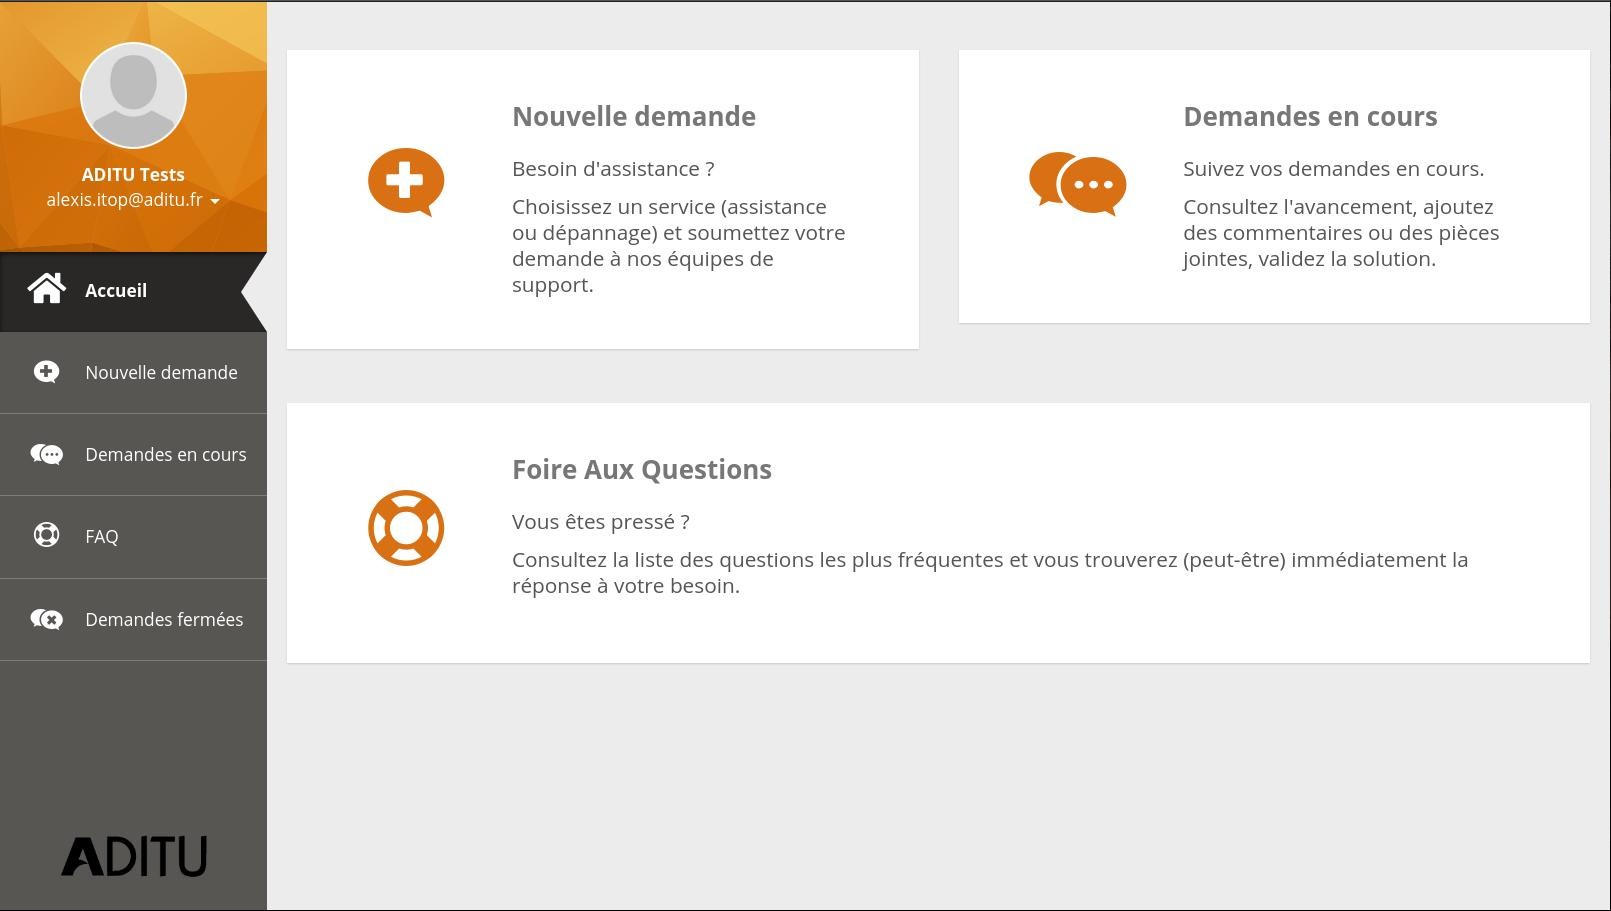
\includegraphics[width=\textwidth - \textwidth / 10]{ressources/images-itop/00.jpg}
    %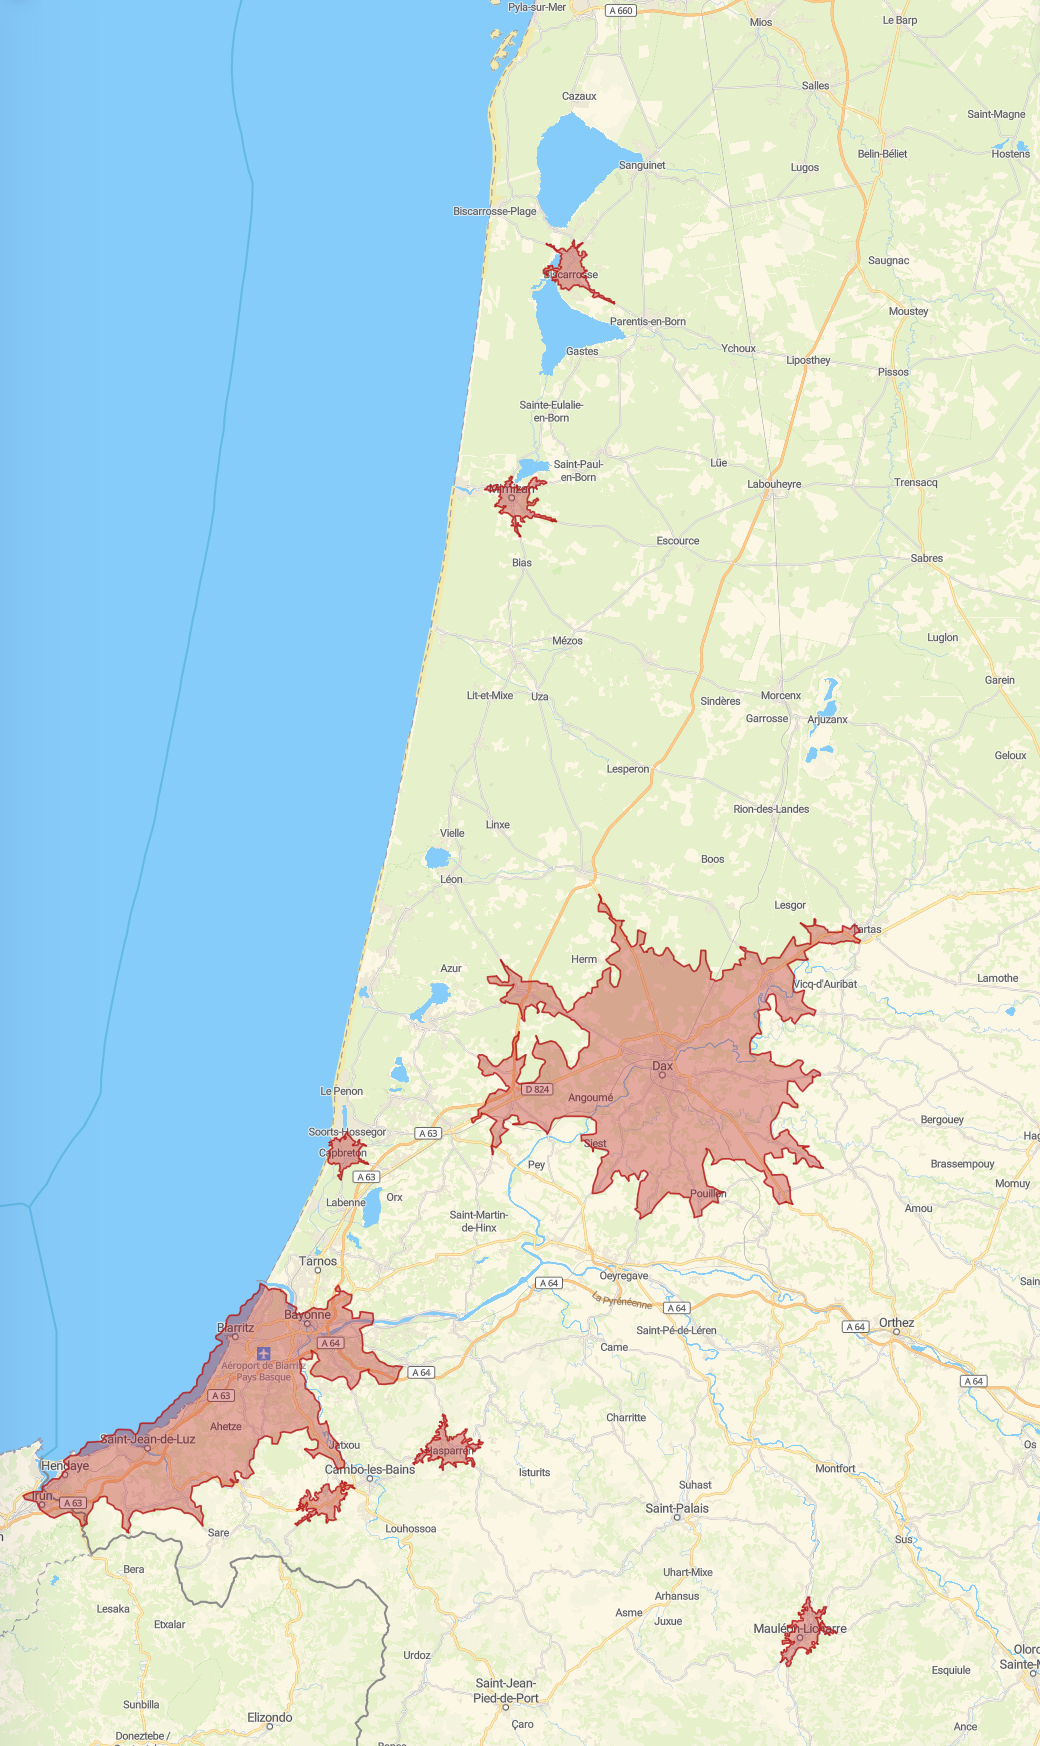
\includegraphics[scale=0.2]{zone_chalandise_aditu.png}
    \figurename
    \caption{Arrivée du client sur l'interface de support}
    \label{fig:00-itop}
\end{figure}

\begin{figure}[H]
    \centering
    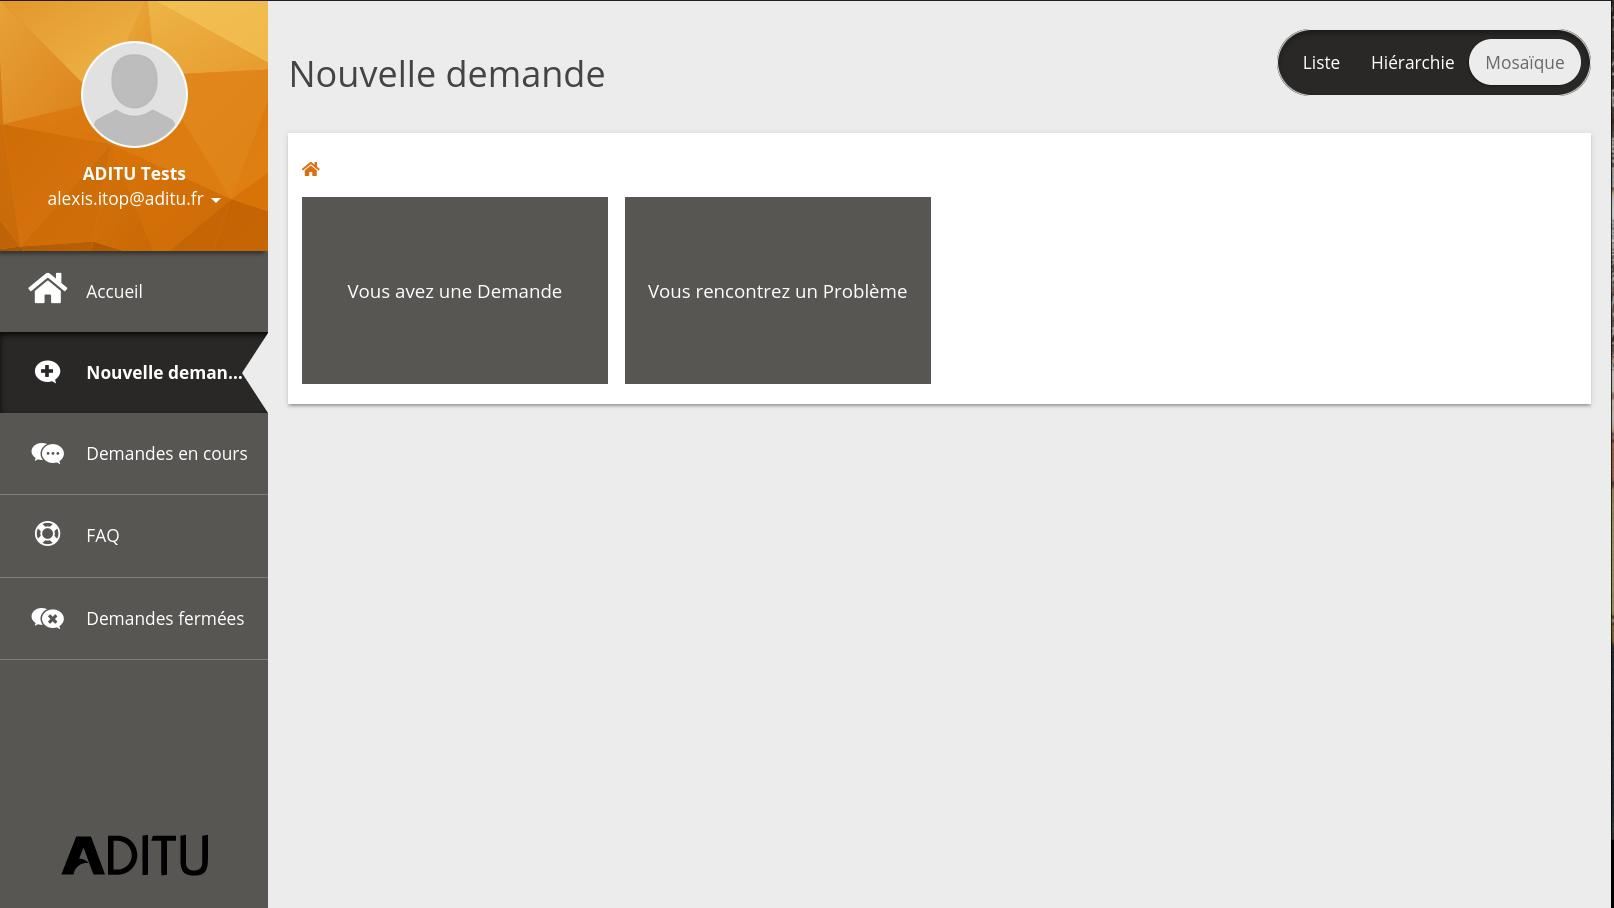
\includegraphics[width=\textwidth - \textwidth / 10]{ressources/images-itop/01.jpg}
    %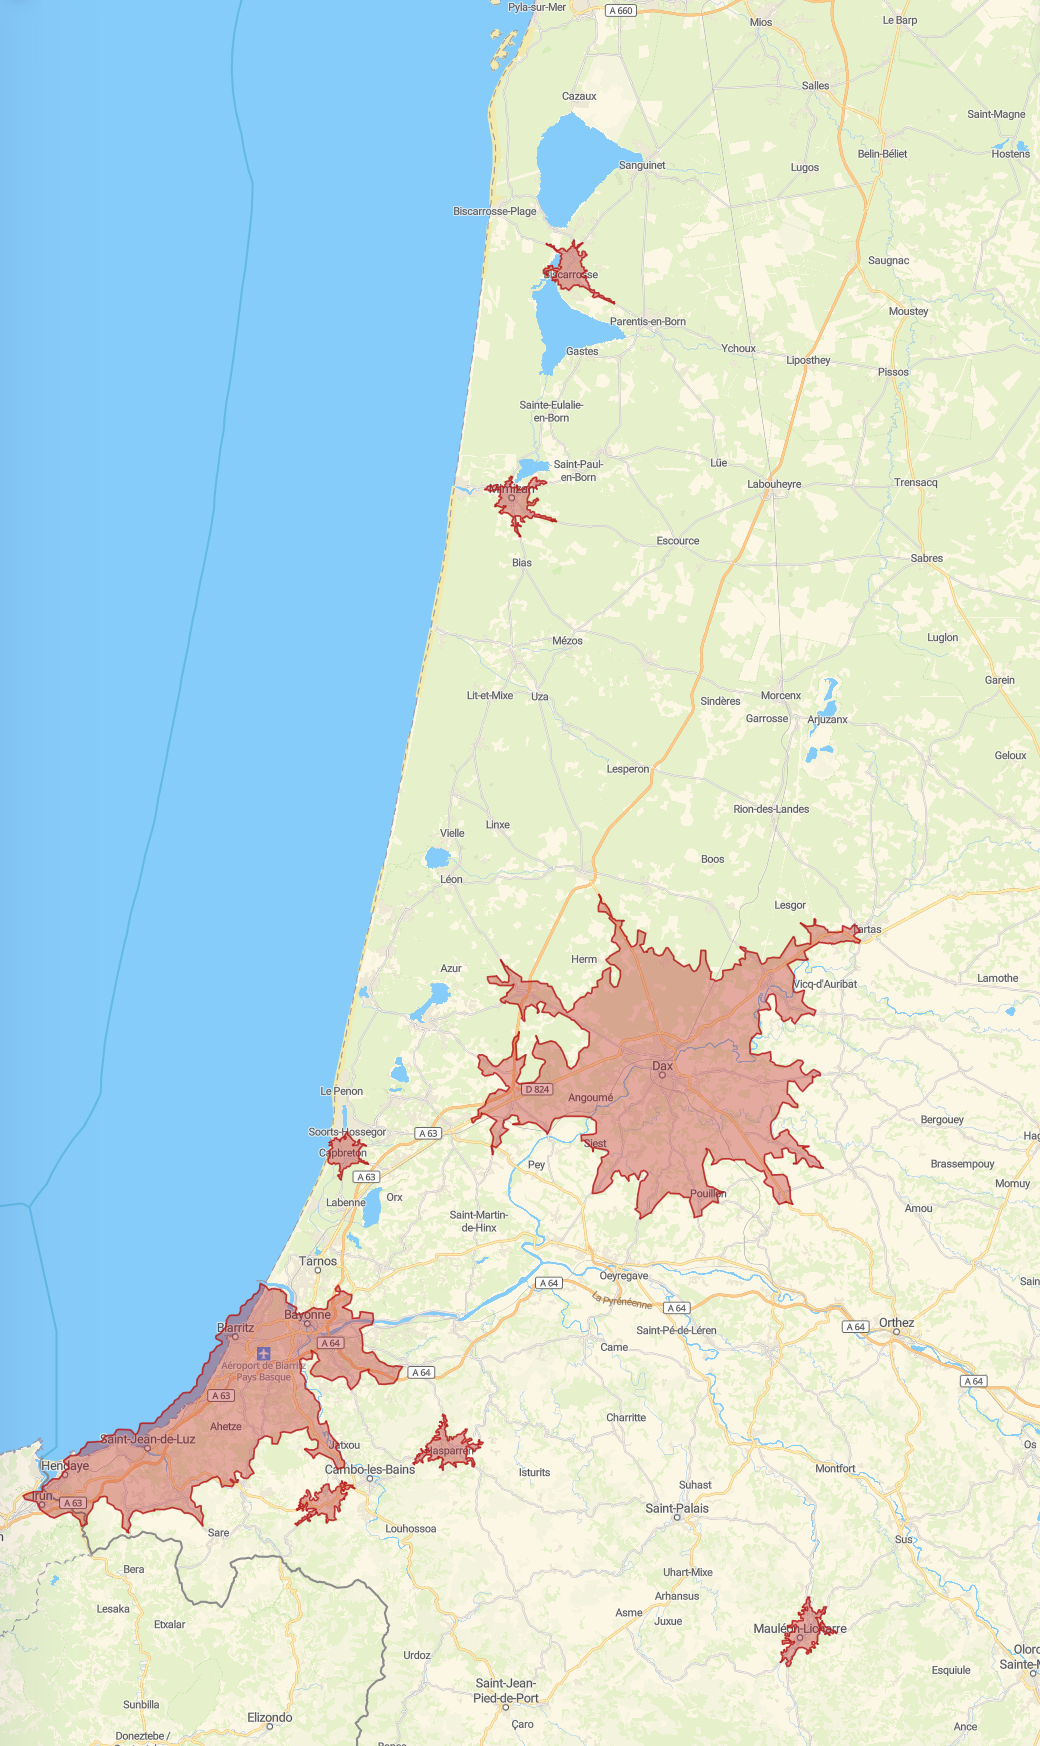
\includegraphics[scale=0.2]{zone_chalandise_aditu.png}
    \figurename
    \caption{Le client souhaite formuler une demande ou un incident}
    \label{fig:01-itop}
\end{figure}

\begin{figure}[H]
    \centering
    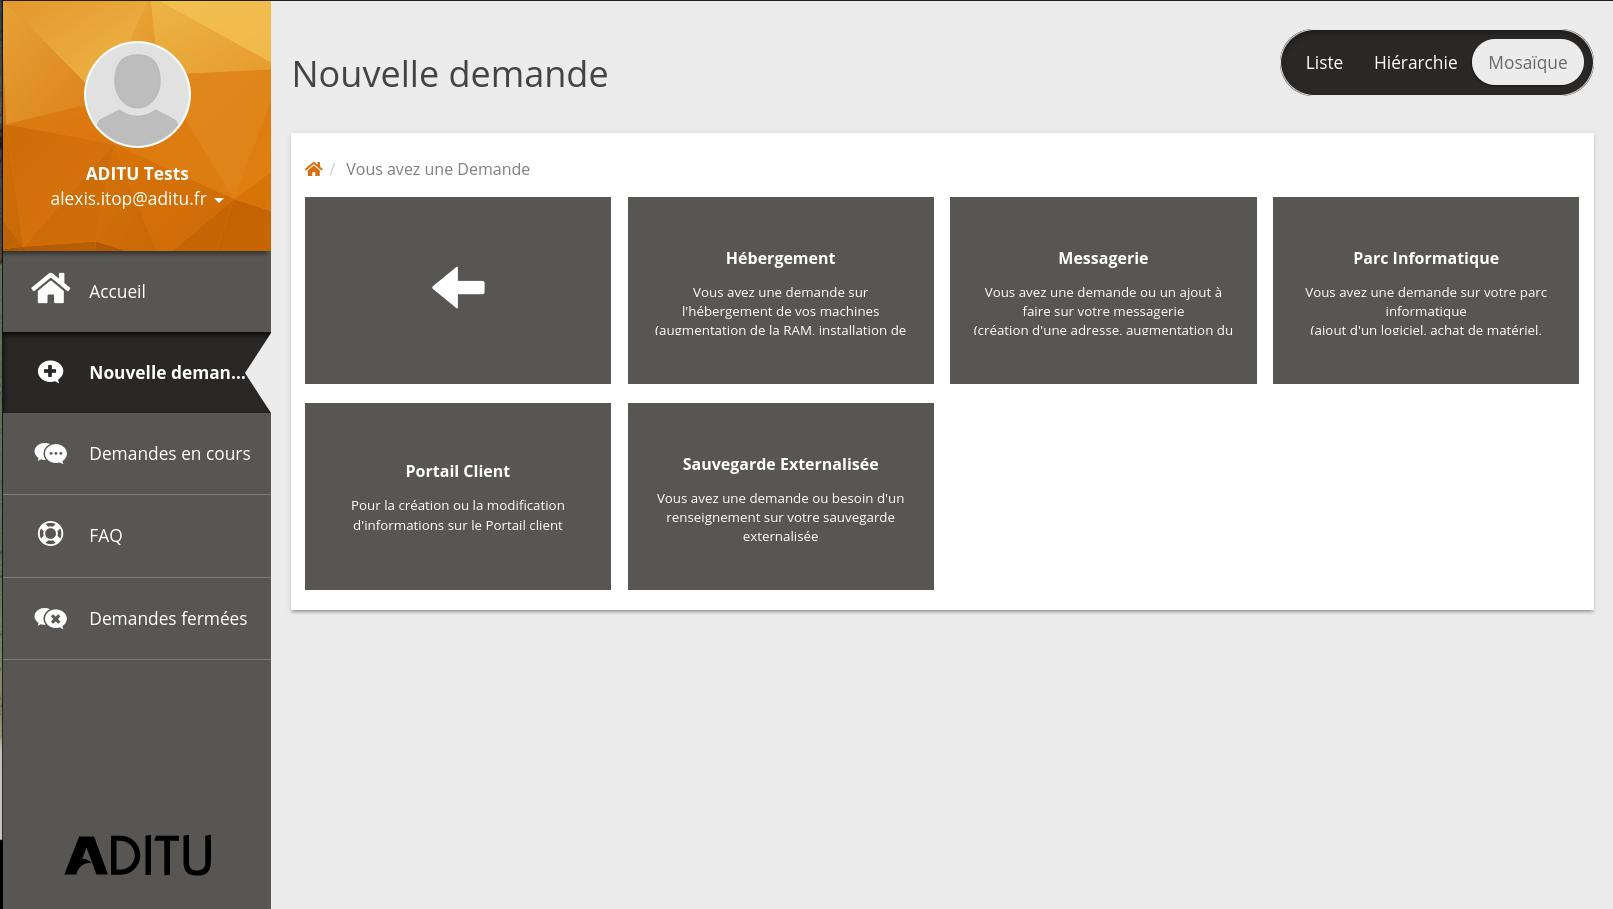
\includegraphics[width=\textwidth - \textwidth / 10]{ressources/images-itop/02.jpg}
    %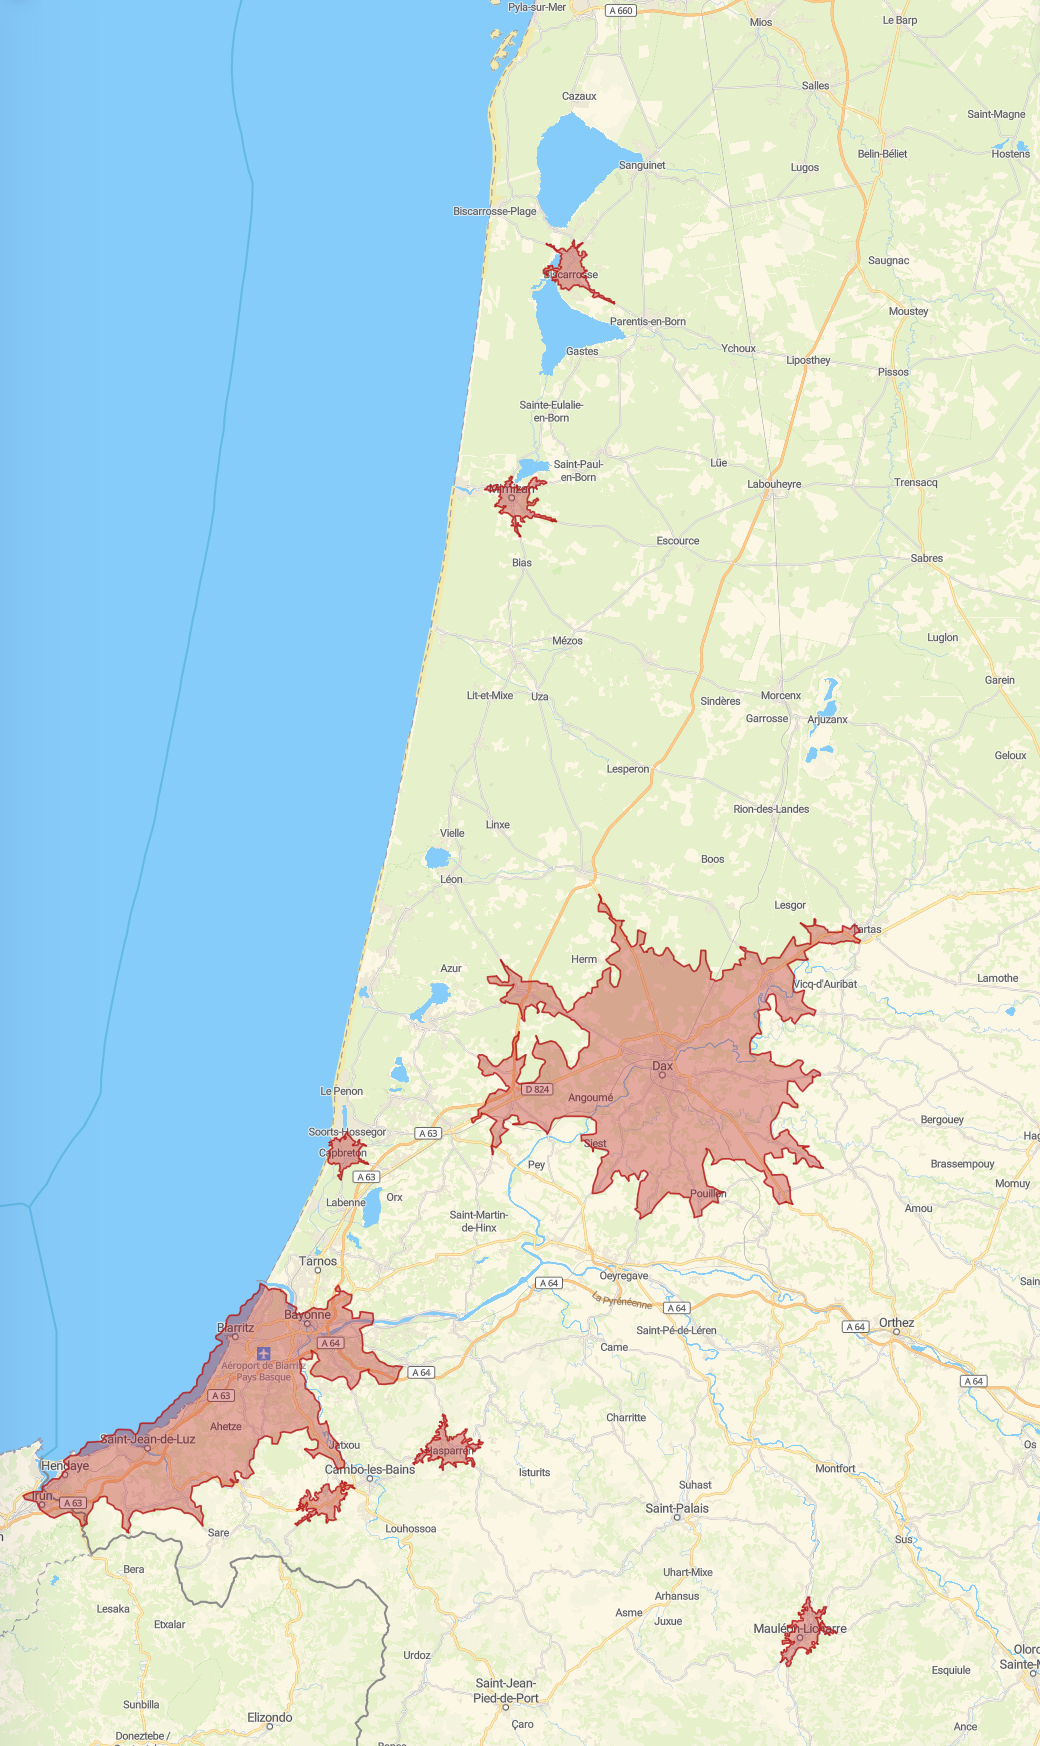
\includegraphics[scale=0.2]{zone_chalandise_aditu.png}
    \figurename
    \caption{Le client choisit le services touché par sa demande (ici, il a beaucoup de services associés)}
    \label{fig:02-itop}
\end{figure}

\subsection{Définition d'un espace d'échange d'informations}

Lors de la préparation, une discussion faisait débat sur l'applicatif : faut-il définir une FAQ \textit{Foire Aux Questions} pour les utilisateurs qui utilisent l'interface (de tout niveau) et/ou un KB \textit{Knowledge Base} pour recueillir les informations pratiques et des procédures à suivre pour certains problèmes des clients.
\\ \\
Chacun comporte ses avantages et ses inconvénients. L'équipe a décidé de garder une FAQ, car elle n'a pas à être trop régulièrement être maintenue , aussi parce qu'elle n'est pas vouée à devenir obsolète dans le temps à contrario d'une KB. Celle-ci s'adresse d'autant plus à un plus grand public, pouvant être lue par beaucoup (pas besoin de compétence techniques, pas de cas par cas...).

\begin{figure}[H]
    \centering
    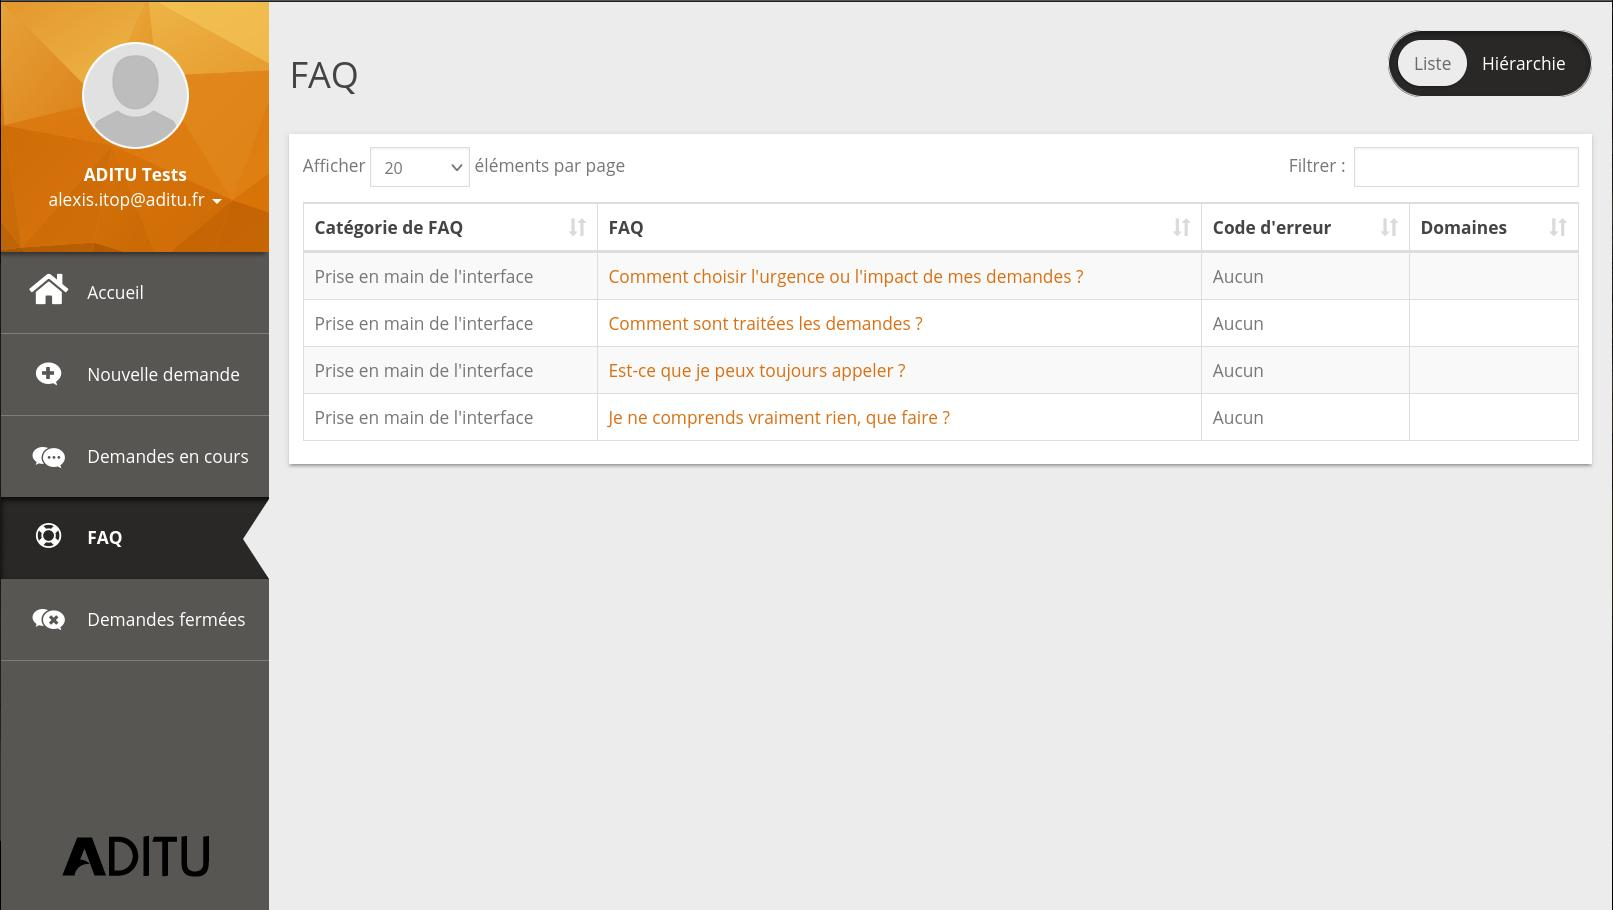
\includegraphics[width=\textwidth - \textwidth / 10]{ressources/images-itop/03.jpg}
    %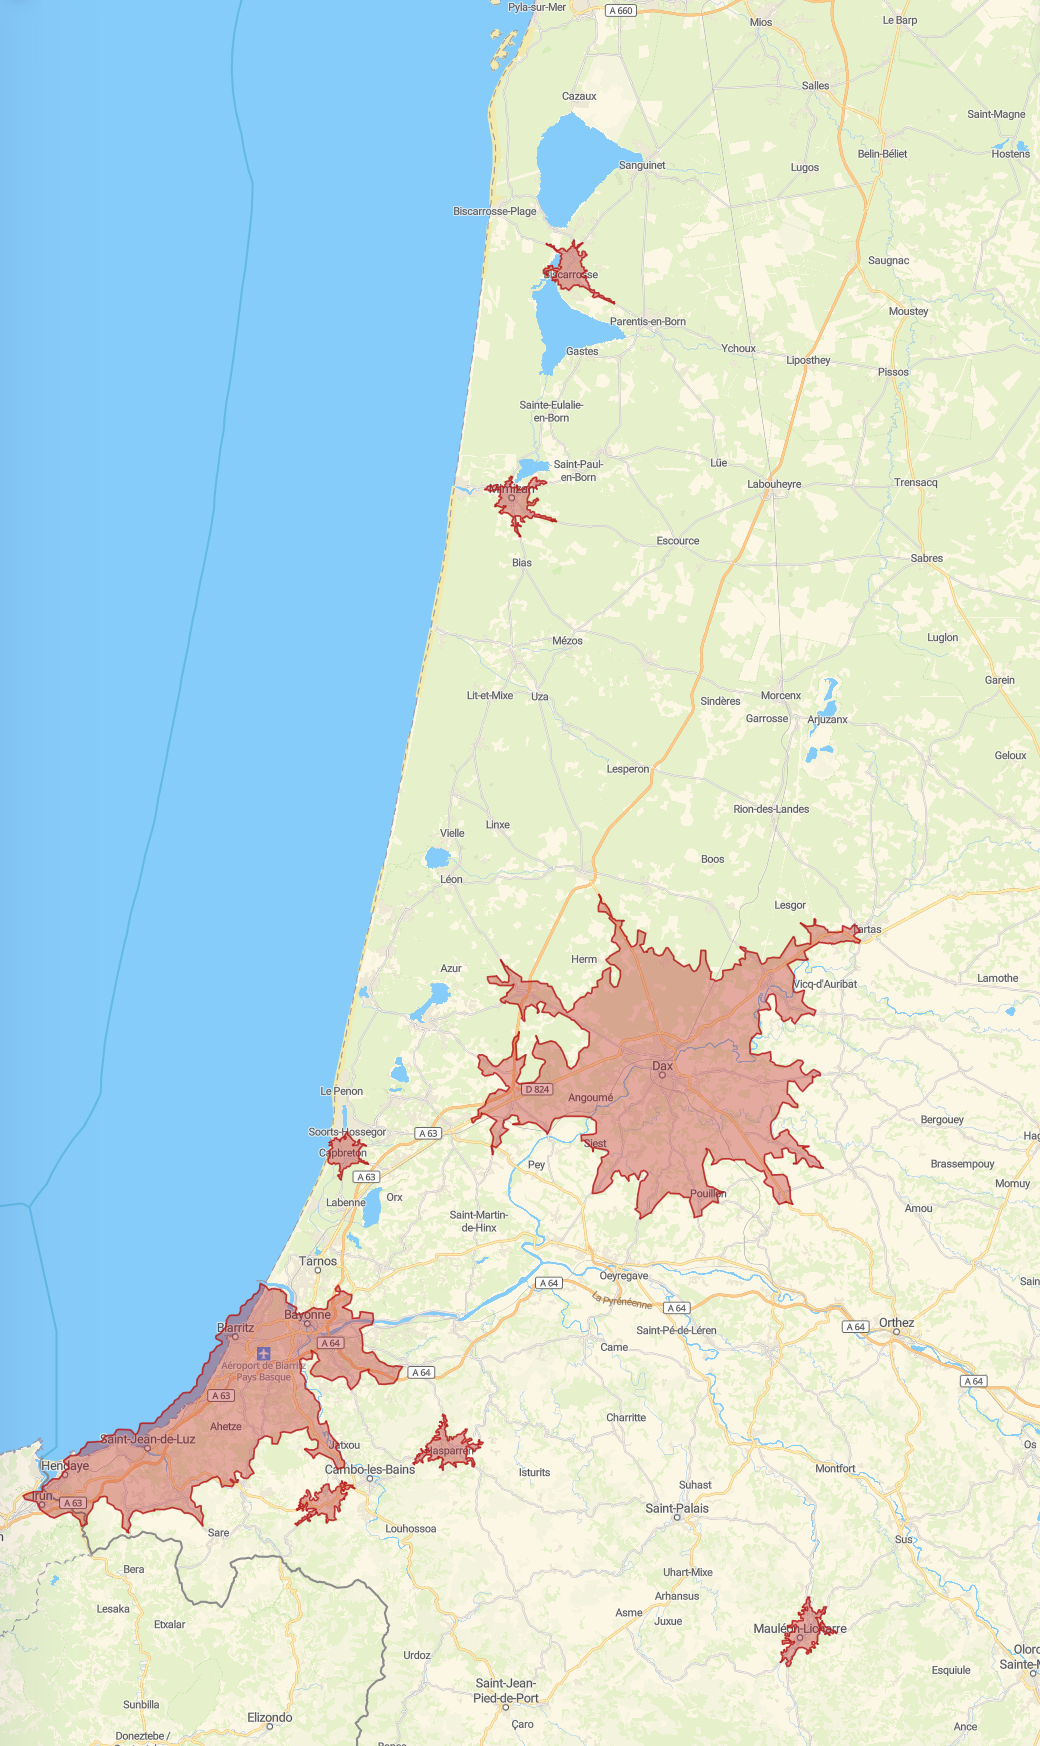
\includegraphics[scale=0.2]{zone_chalandise_aditu.png}
    \figurename
    \caption{Exemple de FAQ présentée au client}
    \label{fig:03-itop}
\end{figure}

\subsection{Application d'un test de charge}

Le dernier test appliqué fut celui d'un test de charge \textit{ou stress test} pour savoir si l'application pouvait répondre à une grande charge (attaque par déni de service, mal fonctionnement, comportement invonlontaire...).
\\ \\
Ainsi, son comportement fut testé lorsque ses ressources matérielles étaient saturées (pouvant provenir du système d'exploitation), lorsque qu'un nombre anormal de tickets sont créés voir le comportement de la base de donnée etc. (toujours attaque par deni de services par rebond sur un compte client).
\\ \\
Tous les tests ont été passés, et suite à une validation de l'équipe, la solution pourra être lancée à mon retour.
    \renewcommand{\figurename}{}
\mychapter{Commencement de l'étude pour une nouvelle solution de supervision}{cap:commencement_etude_supervision} 
\lhead{Commencement de l'étude pour une nouvelle solution de supervision}

Un des sujets majeurs de mon alternance était le changement de l'infrastructure de supervision des équipements d'ADITU et de ses clients. Tout l'intérêt était de comprendre pourquoi ce changement devait s'opérer, comprendre l'infrastructure actuelle, assimiler les précédentes et actuelles techniques de supervision pour enfin commencer une étude comparative de solutions.
\\ \\
Cette étude et les éléments cités précédemment prendront beaucoup de temps. Dans les faits, c'est aussi un alternant qui a monté la solution de supervision actuelle, il a pris une année pour. Mon tuteur et mon responsable m'ont alors conseillé d'y \textit{"aller en douceur"}, pour prendre le temps de comprendre ce que je faisais et pour fournir une solution propre, pour notamment ne pas revenir sur l'élaboration d'une solution comme je le fais actuellement.

\section{Pourquoi un changement de supervision}

ADITU possède un regroupement de supervisions, toutes d'époques différentes. La première supervision est ancienne, opérationnelle et dédiée aux équipements d'ADITU qui fut par la suite reprise pour y ajouter certains clients. Une deuxième supervision a été initiée par l'alternant, regroupant plusieurs solutions, avec certaines pour afficher des statistiques/graphiques... pour les clients.
\\ \\
Le problème de la solution de supervision actuelle est sa disparité (serveurs sur trop de sites différents, trop de solutions différentes sont utilisées...). Sa complexité posant des problèmes lors du maintient, ce qui demande en conséquent beaucoup de temps de travail non valorisé.
\\ \\
Par mon arrivée, ADITU s'est voulu reprendre son projet de supervision en unifiant ses structures, en les documentant davantage et en déclarant des procédures finies pour son maintient. En soit, fournir une nouvelle solution de supervision saine, complète, stable et bien documentée.

\section{Inspection du fonctionnement et de l'état des anciennes solutions}

Une partie continue de mon travail était d'étudier les supervisions en place pour comprendre leur fonctionnement (tunnels sécurisés vers les réseaux des clients, applicatifs ou protocoles de supervision utilisés,paramètres renseignés...). Tout ce travail permet aussi de remettre en question les documentations et procédures existantes pour les solutions en place.
\\ \\
Pour en comprendre le plus possible sur celles-ci, j'ai dû me former à les utiliser afin de pouvoir le mieux que possible les étudier. Je le faisais en montant des laboratoires, dans lesquels j'installais et apprenais à utiliser et en me documentant sur les intuitions que j'avais. Mon apprentissage passais aussi par la recherche dans le code existant des solutions, pour comprendre leur fonctionne et pourquoi elles l'étaient ainsi. Ainsi, j'essayais d'avoir un point de vue le plus global et précis des solutoions.

% L'état : parce que la solution vie, elle change, elle évolue

\section{Apprentissage et documentation des principes de supervision}

Mon étude de l'infrastructure existante s'est coordonnées à mon apprentissage des principes de supervision en entreprise. Par ceux-ci, je me suis alors récolté une gifle d'humilité en effleurant les aspects à considérer pour les solutions de supervision en milieu professionnel. Ainsi, une autre grande partie de mon exercice était aussi la recherche de fonctionnalités et de mouvements de supervision, en me renseignant un maximum sur les méthodes utilisées, les technologies en vogue, pourquoi, et en les questionnant.
\\ \\
Pour la suite de cette section, j'explique certaines notions que je trouvais intéressantes à souligner pour ce document. Un hôte distant/supervisé sera la machine sur laquelle l'on souhaite observer des métriques \textit{informations à superviser}. Pour les données publiques (accessibilité d'un site WEB... accessibile depuis Internet), la collecte de métriques peut se faire sans authentification; pour d'autres informations internes ou sensibles (utilisation des ressources, vérification de configurations...) un agent ou protocole doit être installé ou configuré sur la machine hôte pour communiquer avec la machine de supervision et lui informer à elle seule de ces informations.
%\\ \\
%J'expose ici certaines notions que je trouve importantes que j'ai apprises durant cet apprentissage.

\subsection{Supervision passive et active}

Le choix d'une solution de supervision active ou passive peut restreindre le choix final de solutions, définissant la méthodologie d'approche de la supervision des hôtes.
\\ \\
Pendant longtemps, la supervision se produisait uniquement dans le sens actif.

\begin{itemize}
    \item[1.] La machine de supervision initiait une demande pour récupérer les métriques d'un hôte (accessibilité, disponibilité d'un site WEB, charge d'utilisation du processeur...).
    \item[2.] L'hôte distant, par le biais d'un agent installé ou d'un protocole adapté, renvoyait une réponse à ces demandes (Echo REPLY, status 200 HTTP/S, moyenne d'utilisation des coeurs de son processeur...).
    \item[3.] La machine de supervision recevait puis interprétait ces informations en (modification de l'état d'un service ou de l'état de l'hôte, remontée d'une alerte...).
\end{itemize}

\noindent Ce modèle de supervision actif propose un modèle de résolution des métriques proactif (la machine de supervision va chercher l'information, pour attendre son retour et interpréter son résultat). Les problèmes de ce modèle sont qu'une communication dans les deux sens doit être initiée pour toutes les machines à superviser et que la machine de supervision doit planifier ses demandes en plus de traiter les informations qu'elle reçoit par la suite. De plus, les machines distantes ont un port ouvert constamment en écoute, problème pour l'exposition si mal sécurisé ou vulnérabilité découverte.
\\ \\
L'agent installé sur l'hôte distant est passif, il ne fait qu'attente les instructions de la machine de supervision. Nous pouvons cependant réfléchir dans l'autre sens, en renvoyant cette fois l'agent installé sur la machine supervisée en actif, la machine de supervision serait passive en attente du signalement. Cela corrige certains problèmes vus précédemment. C'est le principe de la supervision passive (point de vue de la machine supervision).
\\ \\
Le modèle de supervision passif se déroulant en suivant.

\begin{itemize}
    \item[1.] L'agent envoie périodiquement ses métriques à la machine de supervision (accessibilité, disponibilité d'un site WEB, charge d'utilisation du processeur...).
    \item[2.] La machine de supervision reçoit et interprète ces informations (modification de l'état ou d'un service de l'hôte, remontée d'une alerte...). \textbf{selon qu'elle reçoit ces métriques ou non}.
\end{itemize}

\noindent Le modèle de supervision passif permet d'initier un communication dans un sens uniquement (réduction du trafic), de protéger les hôtes en n'exposant pas de port (pour en exposer uniquement celui de la machine de supervision uniquement - plus simple à protéger que 500 interfaces d'hôtes, réduisant la surface d'attaque d'un parc...).
\\ \\
Cependant, la méthode d'interprétation passe de proactif à réactif (on interprète selon ce qu'on reçoit ou ce que l'on ne reçoit pas). Une décision importante à prendre est de savoir s'il nécessaire d'installer une solution de supervision réactive ou proactive (à définir selon les besoins, l'infrastructure déjà existantes, la disposition des pare-feux pour l'ouverture de port et l'observation du traffic, la criticité de la structure, la sécurité demandée, les actions possibles sur les hôtes...).

\subsection{L'alerting, la supervision et les statistiques}

Lorsque je manipulais des solutions de supervision en essais, en les utilisant et sans le remarquer, celles-ci tendaient à regrouper trois très grandes responsabilités dans leur utilisation. Que sont la supervision des métriques, l'interprétation en graphique et/ou de la corrélation d'événements et l'alerting pour informer les administrateurs des potentiels problèmes.
\\ \\
Je n'ai vu qu'extrêmement peu d'articles, de blogs ou de forums remarquer de cette différenciation, même pour ceux les plus récents. L'intérêt des \textit{nouvelles générations de supervision} est de pouvoir changer les briques de sa solution quand on le souhaite et par ce que l'on souhaite, afin d'isoler les responsabilités, de changer uniquement certaines parties sans avoir à changer de solution, être réutilisables etc. En résulte une solution très permissive, tolérante au changement et non restrictive à l'utilisation dû à la sectarisation des responsabilités.
\\ \\
Les anciennes solutions de supervision tendent à vouloir tout faire par elles-mêmes (Nagios, Centreon, Checkmk, Zabbix, Icinga, Shinken...). Alors que les solutions en vogues tendent à se spécifier dans leur tâche pour permettre d'être facilement remplacées ou tolérantes aux problèmes, en séparant la métrologie de la collecte d'information, des bases de données... Cela est notamment rendu possible grâce à la démocratisation de l'utilisation de conteneurs, et aux solutions d'orchestration comme Kubernetes pour n'en citer qu'un. Pour ne citer que certaines briques de cette \textit{nouvelle génération} : Prometheus pour l'export des données, Grafana leur interprêtation, InfluxDB une base de donnée spécialisée dans le stockage de métriques, pareil pour Victoria Metrics, Loki pour l'export cette fois des journaux d'activités, Tempo pour la correlation d'événements, Mimir solution de stockage pour Prometheus...
\\ \\
En résulte un retour en arrière chez les administrateurs et architectes informatiques et réseaux : ils souhaitaient payer une licence pour tout faire, désormais ils souhaitent avoir leur solution personnalisée à leurs besoins la plus polyvalente possible, en utilisant des outils comem Docker pour leur supervision et pouvoir ajouter ou remplacer des briques comme ils le souhaitent.

\subsection{Maintient de la charge, rétention, expansibilité et distributivité}

Certaines notions sont cruciales pour une solution de supervision en environnement de production : le maintient de la charge d'informations, la rétention des métriques collectées, sa capacité d'expansion et celle à être distribuée en plusieurs endroits en sont des exemples.
\\ \\
Il est essentiel pour une supervision de pouvoir interpréter dans un temps imparti les informations qu'elle reçoit : auquel cas, celle-ci créera une pile de métriques en attente de traitement, qui elle-même sera submergée par la quantité de métriques qui arrivera par la suite. Le maintient de la charge désigne toutes les techniques en place pour garantir le traitement de chaque flux de données à tout moment de la journée et de la nuit, selon toutes circonstances (de 1000, 10000 hôtes non réguliers dans la journée). Dans certains cas précis, des administrateurs ne peuvent pas se permettre de ne pas voir certaines informations à cause d'un mauvais dimensionnement.
\\ \\
Pour des raisons juridiques et judiciaires, les entreprises du secteur du numérique françaises sont dans l'obligation de journaliser leurs informations en cas d'appel à consultation dans le cadre d'affaires judiciaires, juridiques et autre sur le sol français. En dehors de cette obligation, il est contingeant de prévoir un plan de rétention des informations et métriques collectées pour de l'étude et de la corrélation d'événements, de la comparaison, de la métrologie, et pour l'appel à consultation des utilisateurs (définit par la RGPD \textit{Règlement Général sur la Protection des Données}). Cet aspect n'est à surtout pas négliger pour une entreprise d'hébergement et de prestation de services informatiques comme ADITU.
\\ \\
Il est aussi essentiel de penser à l'expansibilité de sa solution de supervision, celle-ci évolue et pourrait être menées à accueillir beaucoup plus d'hôtes à superviser (arrivée d'un client, ajout d'un bâtiment ou expansion...). Une solution de supervision se doit d'être expansible horizontalement (ajout de machines pour de la répartition de charge...) et de proposer si nécessaire un plan de distribution de charge.
\\ \\
Certaines solutions, à leur échelle, ont besoin d'être distribuées. Dans l'exemple d'ADITU, celle-ci sera centralisée à Dax dans le data centre de DATA3, mais sera distribuée chez ses clients : une plus petite machine de supervision récupérera les données du réseau local chez un client, pour en envoyer le condensé des métriques récupérées à la machine de supervision centrale à Dax. Cela permettra de ne pas consommer trop de bande passante du réseau client pour Internet, en centralisant et compressant les métriques. Cela garantira aussi l'intégrité des données, restant intactes en cas de coupure d'un lien vers Internet ou une indisponibilté, d'atténuer le problème de latence entre sites et d'initier une vision de distribution de charge - déchargeant petit à petit la supervision centrale du traitement de toutes les données. Cette notion n'est pas discutable pour des solutions de supervision intercontinentales ou internationales.

\section{Premières intégrations et études comparatives}

Un autre moyen d'apprendre continuellement est de le faire par soi est au travers d'un laboratoire pour essayer ses intuitions en prenant main sur les solutions. En appliquant mes idées ou celles d'autres personnes, mon apprentissage s'est enrichi grandement en touchant les problèmes réels que j'aurai pu rencontrer en environnement de production.
\\ \\
J'ai trouvé que toutes les solutions étaient extrêmement différentes dans leur fonctionnement, dans leurs fonctionnalités ou dans leur modèle de économique : j'ai décidé de les comparer sur ce qu'on attend d'elles plutôt que de les comparer sur ce qu'elles proposent individuellement pour pouvoir les départager. Ainsi, je ne recherche pas la meilleure solution mais celle qui répondra au mieux à nos besoins.

\subsection{Mise en étude des solutions}

J'ai monté les solutions suivantes après repérages et conseils pour commencer mon étude en cas pratique : Nagios, Centreon, Checkmk, Netdata et Zabbix. Je rappelle que mon objectif n'est pas d'aller rechercher les applications avancées de ces solutions mais de voir comment celles-ci répondraient à nos besoins, voir leurs intégrations pour les étudier ensuites.
\\ \\
J'ai essayé pour chacune de comprendre l'idée générale derrière leur fonctionnement et d'observer leurs limites dans l'environnement dans lequel nous souhaitions les intégrer. J'espère toujours aujourd'hui avoir vu un maximum de choses utiles dans un temps restreint pour chacune, de ne pas avoir fait fausse route sur certaines de leurs fonctionnalités ou intégrations.

\subsection{Point rapide sur chacune des solutions mises à l'épreuve}

Nagios est une solution connue, stable, et extrêmement pratique dans sa gestion par ses fichiers \texttt{*.cfg}. Sa syntaxe est agréable, mais son talon d'Achille reste son interfaçage pour sa version Core : il a besoin de solutions externes. Des intégrations existent mais complexifient l'installation, déjà en vogue actuellement chez ADITU.
\\ \\
Centreon est un fork \textit{une copie est basée sur} de Nagios, intégrant les mêmes fonctionnalités avec un front-end \textit{interfaçage utilisateur} acceptable. Cependant, celui-ci restreint les intégrations propres possibles par son modèle de financement et ne correspond pas au cahier des charges demandé sur certains points...
\\ \\
Checkmk est aussi un fork de Nagios, mais pour moi celui-ci est trop jeune et pas assez déployé pour avoir sa place dans un milieu de production. On perd aussi beaucoup en simplicité en l'utilisant et de support par manque de communauté.
\\ \\
Netdata est un outil formidable pour de la surveillance en tant réel de charge, et il est même selon moi le meilleur pour de la métrologie. Cependant, il n'est pas fait pour de la supervision (scripts personnels, intégrations) ou de la remonté d'alertes (alerting).
\\ \\
Zabbix est l'entre-deux le plus intéressants : énormément d'intégrations, un modèle financier pas trop restrictif et une métrologie correcte. Il n'en reste cependant pas aussi simple que Nagios, où intégralement tout peut se faire intuitivement en lignes de commandes. Il répond à l'intégralité du cahier des charges, ce serait la solution à choisir basée sur les problèmes initiaux à répondre.
    \mychapter{Annexes}{cap:annexes}
\lhead{Annexes}

Regroupement des documents servant à l'appui des éléments cités précédemment. Pouvant être de toutes formes (images, blocs de texte, photos...).

\section{Cahier des charges supervision}

Cahier de charges supervision

La recherche de solution applicative de supervision devra se base au
minimum sur deux applications pour avoir une comparaison objective.

Voici les fonctionnalités souhaitées~:

\ul{Serveurs Proxy}

L'utilisation de \textbf{SERVEUR PROXY} pour ne pas avoir un seul
serveur qui se charge de l'ensemble de vérifications de sonde.

\ul{DASHBOARD}

Un \textbf{DASHBOARD UNIQUE} qui inclut l'ensemble des serveurs de
supervision.

\ul{DASHBOARD TV}

Un \textbf{DASHBOARD} pour la télé qui liste les notifications de la
plus récente a la plus ancienne. (Comme celle que l'on a actuellement.)

\ul{Type de contrôles}

L'application devra gérer les contrôles \textbf{PASSIF} et
\textbf{ACTIF} et la prise en charge des contrôles via \textbf{SNMP}.

\ul{Type de paramétrages}

La possibilité de configurer les hosts via l'interface graphique et via
les fichiers de configuration.

Exemple~: sur l'ancienne supervision on créer un fichier de conf par
client.

\ul{Notifications}

Les notifications devront être effectuées par mail et par SMS tout en
ayant une gestion des utilisateurs et des groupes (possibilité
d'intégrer la solution à notre serveur d'SMS)

Déplacer le GSM dans le bureau ADITU de Pulseo pour une meilleur
couverture réseau (prévoir onduleur + switch mangeable)

\ul{Accès restreint client}

Donner la possibilité à certains clients de visionner leur supervision
en lecture et d'être alerté par mail.

\ul{Graphique}

Côté graphique, il serait bien que la solution puisse avoir la
possibilité d'inclure les graphiques comme fait Cacti pour éviter
d'avoir 2 solutions.

\begin{itemize}
\item
  Graphique réseau
\item
  Graphique volumétrie disque pour voir l'évolution du stockage
\item
  Graphique mémoire ou CPU
\end{itemize}

\ul{Tarif}

Open source gratuit

% \begin{figure}[H]
%     \centering
%     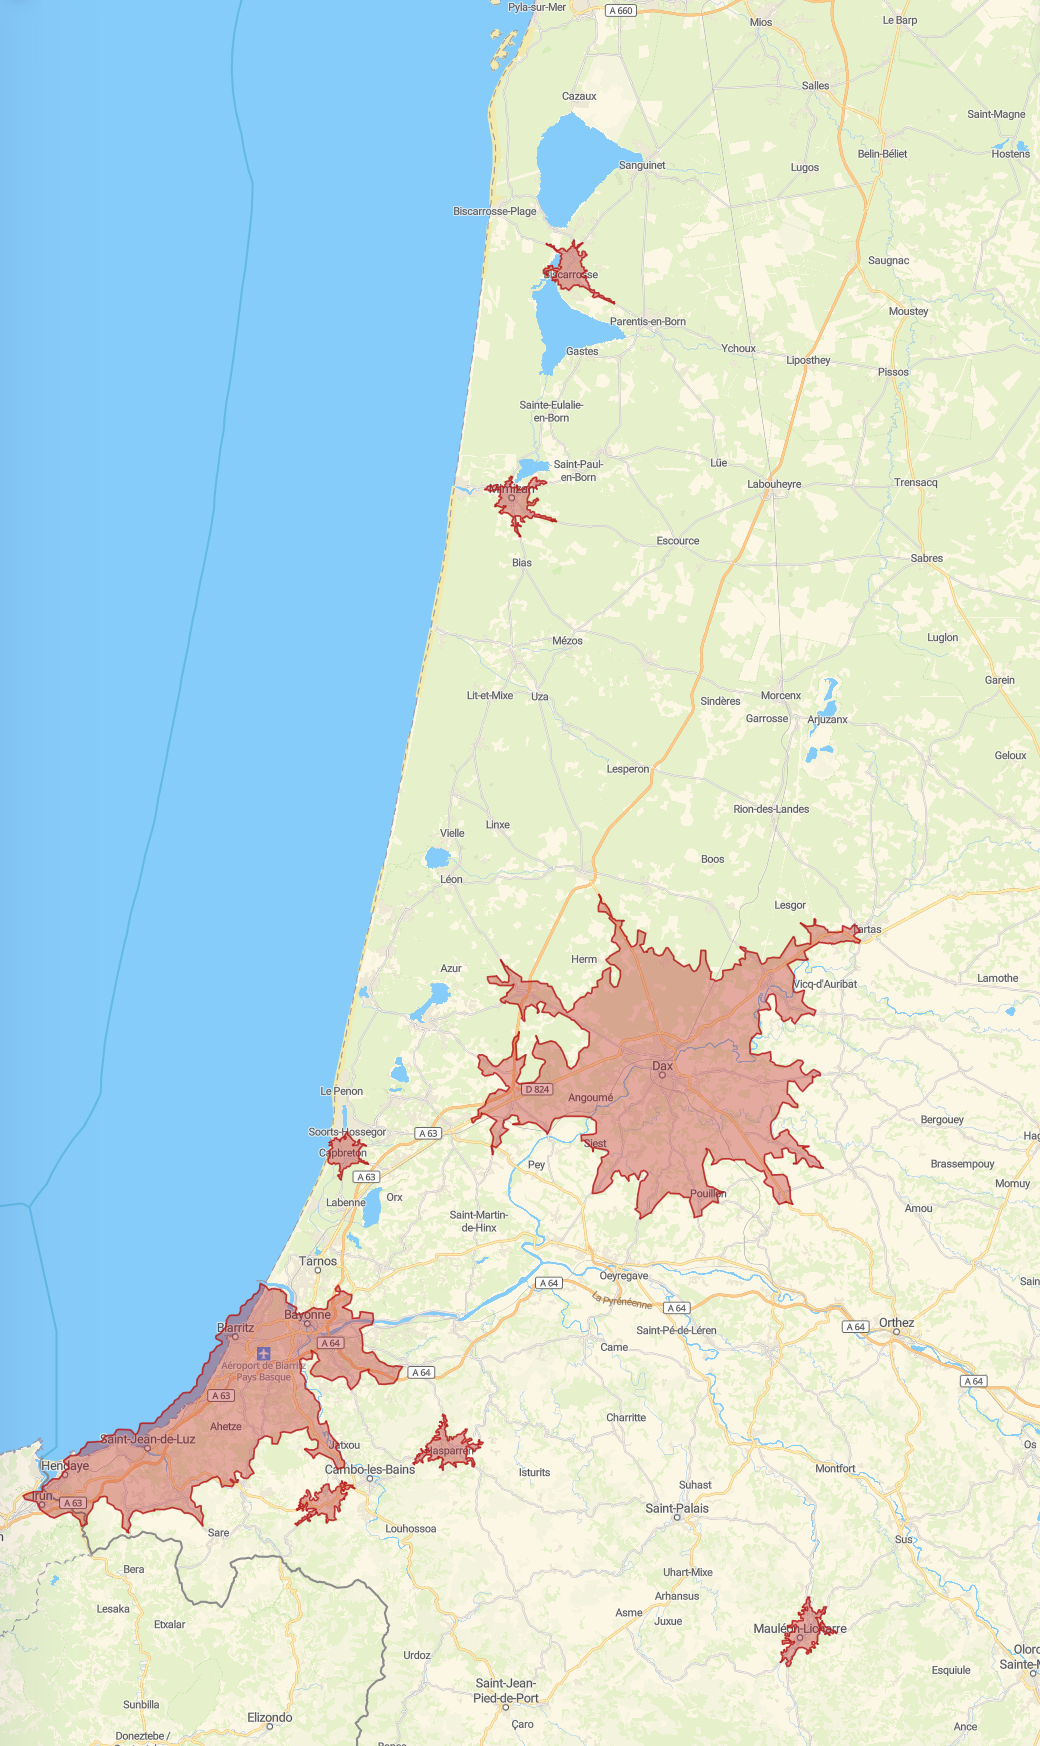
\includegraphics[width=\textwidth - \textwidth / 5]{zone_chalandise_aditu.png}
%     %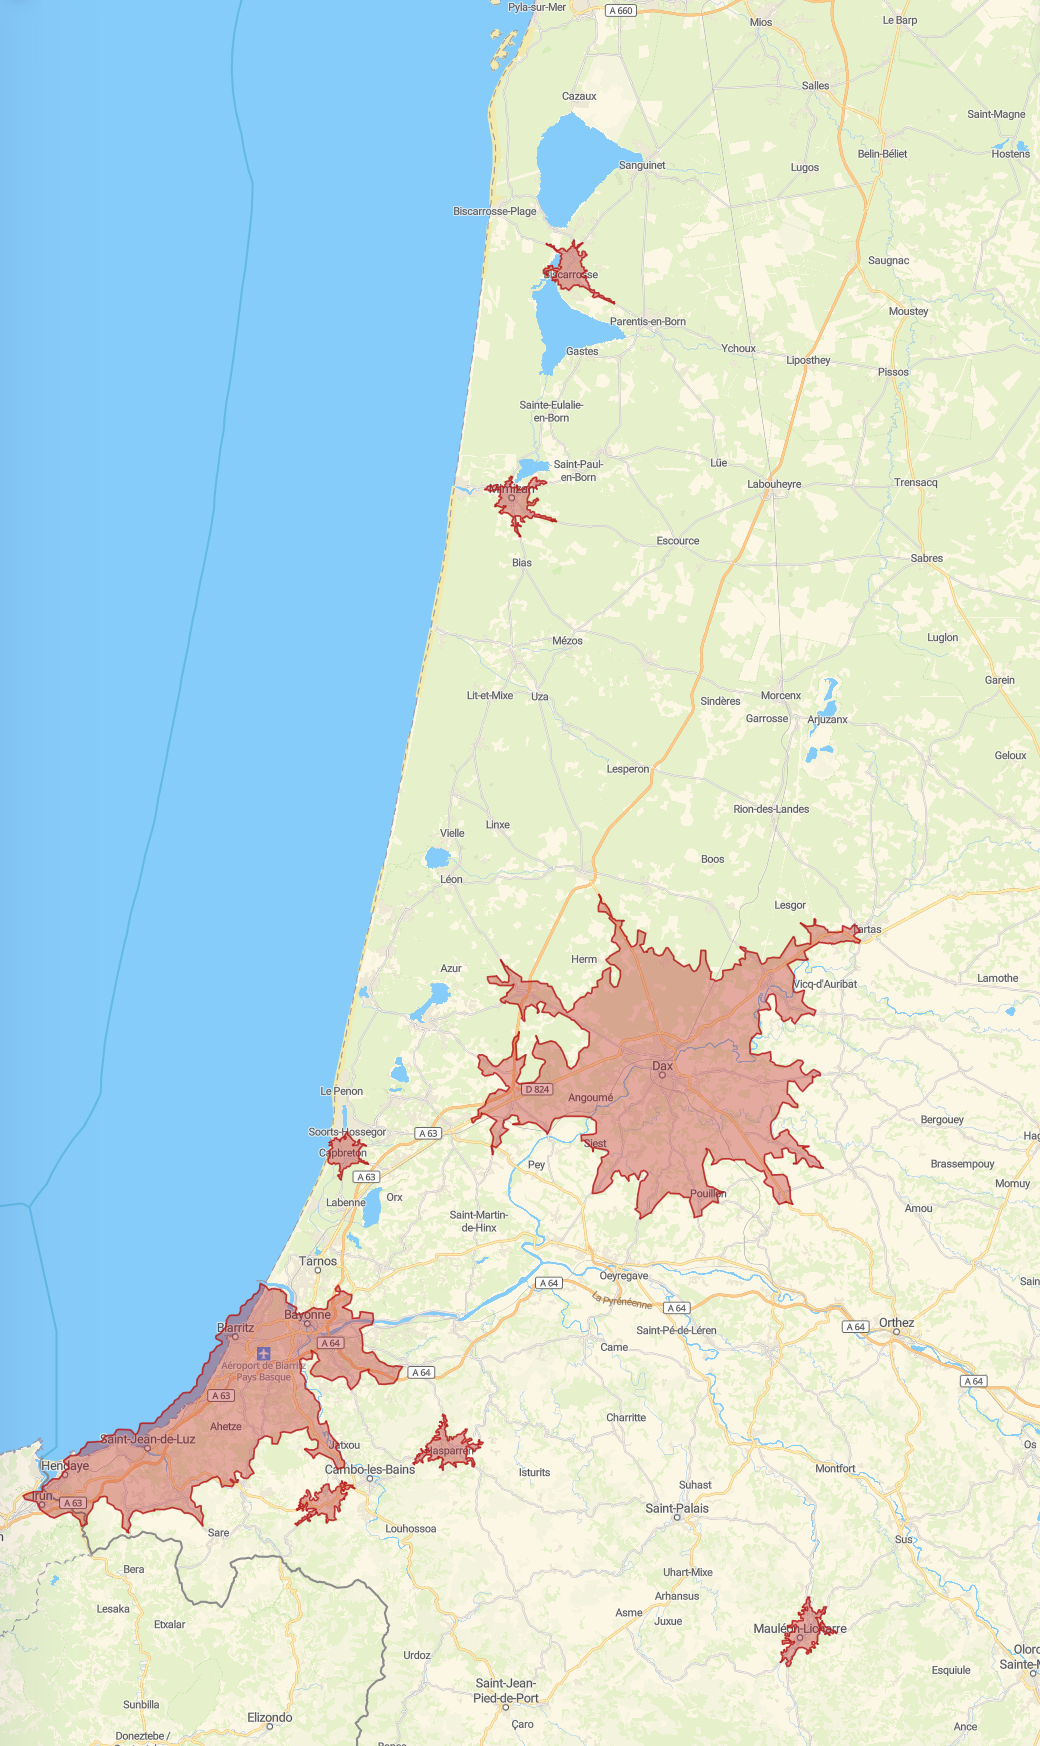
\includegraphics[scale=0.2]{zone_chalandise_aditu.png}
%     \figurename
%     \caption{Visualisation de la zone de chalandise d'ADITU, regroupée autour de ses datacenters à Bidart et à Dax}
%     \label{fig:zone_chalandise}
% \end{figure}

% \section{Cahier des charge Ticketing}

% % \begin{figure}[H]
% %     \centering
% %     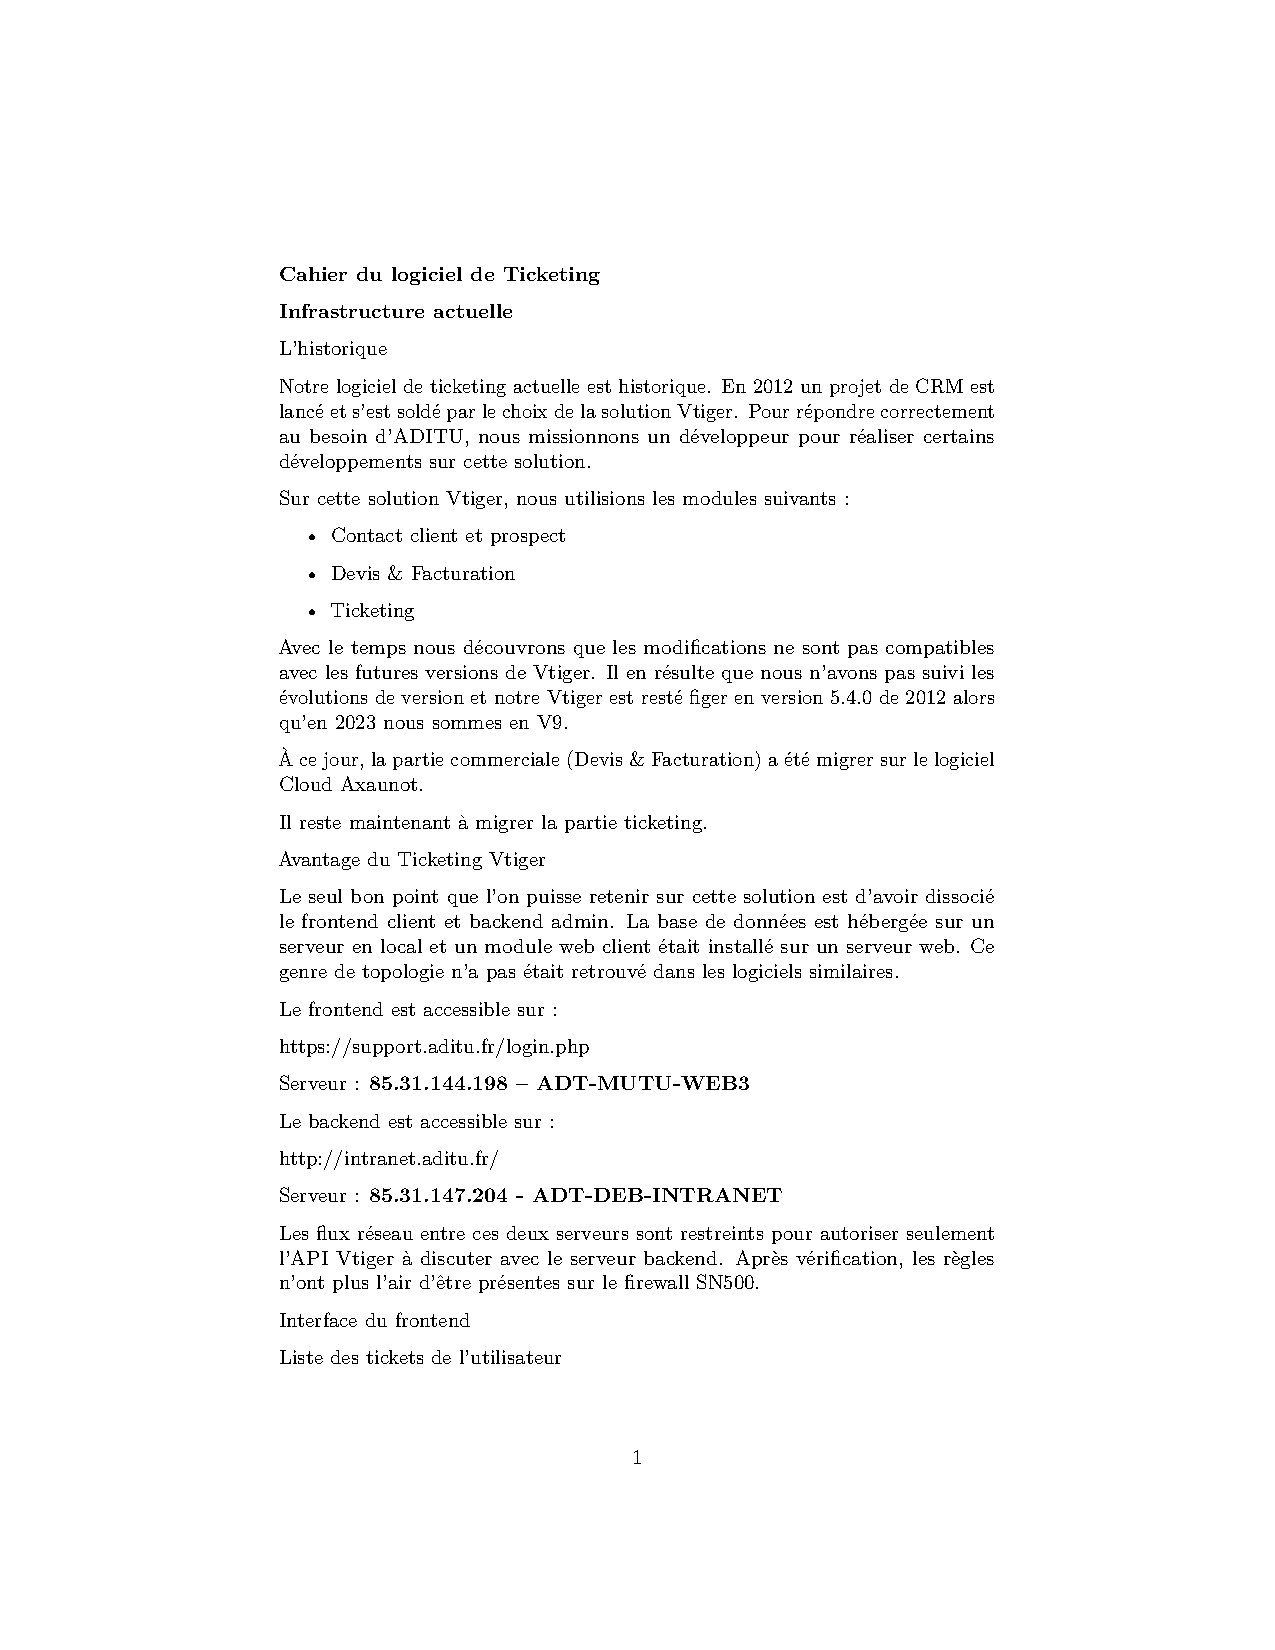
\includegraphics[width=\textwidth - \textwidth / 20]{CDC-Ticketing.pdf}
% %     \figurename
% %     \caption{Fiche de poste de notre alternance}
% %     \label{fig:poste}
% % \end{figure}

% \textbf{Cahier du logiciel de Ticketing}

% \textbf{Infrastructure actuelle}

% L'historique

% Notre logiciel de ticketing actuelle est historique. En 2012 un projet
% de CRM est lancé et s'est soldé par le choix de la solution Vtiger. Pour
% répondre correctement au besoin d'ADITU, nous missionnons un développeur
% pour réaliser certains développements sur cette solution.

% Sur cette solution Vtiger, nous utilisions les modules suivants~:

% \begin{itemize}
% \item
%   Contact client et prospect
% \item
%   Devis \& Facturation
% \item
%   Ticketing
% \end{itemize}

% Avec le temps nous découvrons que les modifications ne sont pas
% compatibles avec les futures versions de Vtiger. Il en résulte que nous
% n'avons pas suivi les évolutions de version et notre Vtiger est resté
% figer en version 5.4.0 de 2012 alors qu'en 2023 nous sommes en V9.

% À ce jour, la partie commerciale (Devis \& Facturation) a été migrer sur
% le logiciel Cloud Axaunot.

% Il reste maintenant à migrer la partie ticketing.

% Avantage du Ticketing Vtiger

% Le seul bon point que l'on puisse retenir sur cette solution est d'avoir
% dissocié le frontend client et backend admin. La base de données est
% hébergée sur un serveur en local et un module web client était installé
% sur un serveur web. Ce genre de topologie n'a pas était retrouvé dans
% les logiciels similaires.

% Le frontend est accessible sur~:

% \url{https://support.aditu.fr/login.php}

% Serveur~: \textbf{85.31.144.198 -- ADT-MUTU-WEB3}

% Le backend est accessible sur~:

% \url{http://intranet.aditu.fr/}

% Serveur~: \textbf{85.31.147.204 - ADT-DEB-INTRANET}

% Les flux réseau entre ces deux serveurs sont restreints pour autoriser
% seulement l'API Vtiger à discuter avec le serveur backend. Après
% vérification, les règles n'ont plus l'air d'être présentes sur le
% firewall SN500.

% Interface du frontend

% Liste des tickets de l'utilisateur

% 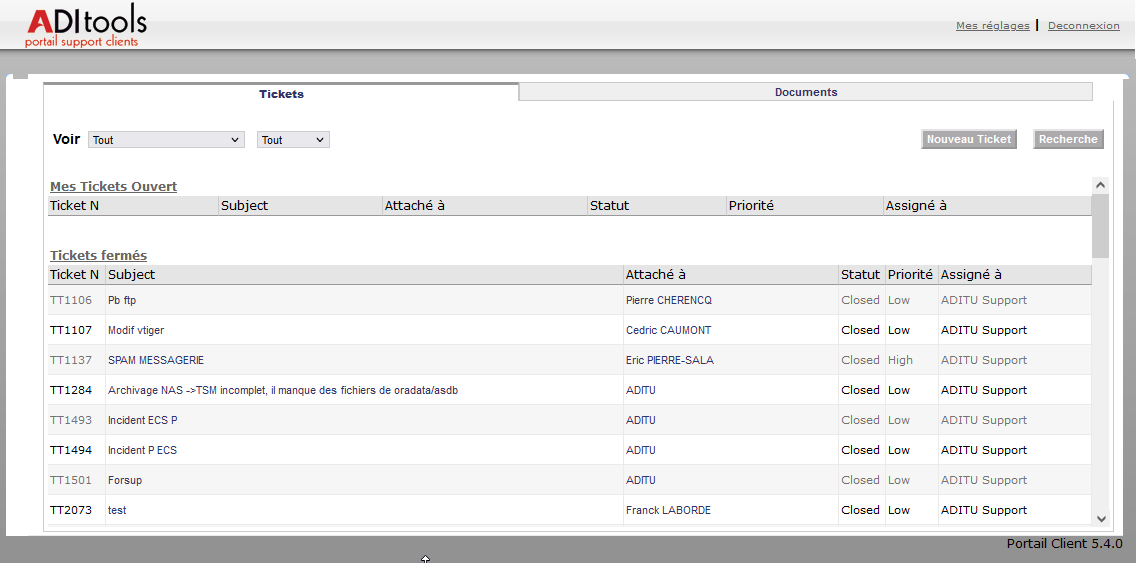
\includegraphics[width=6.3in,height=3.12222in]{image1.png}

% Création de tickets

% 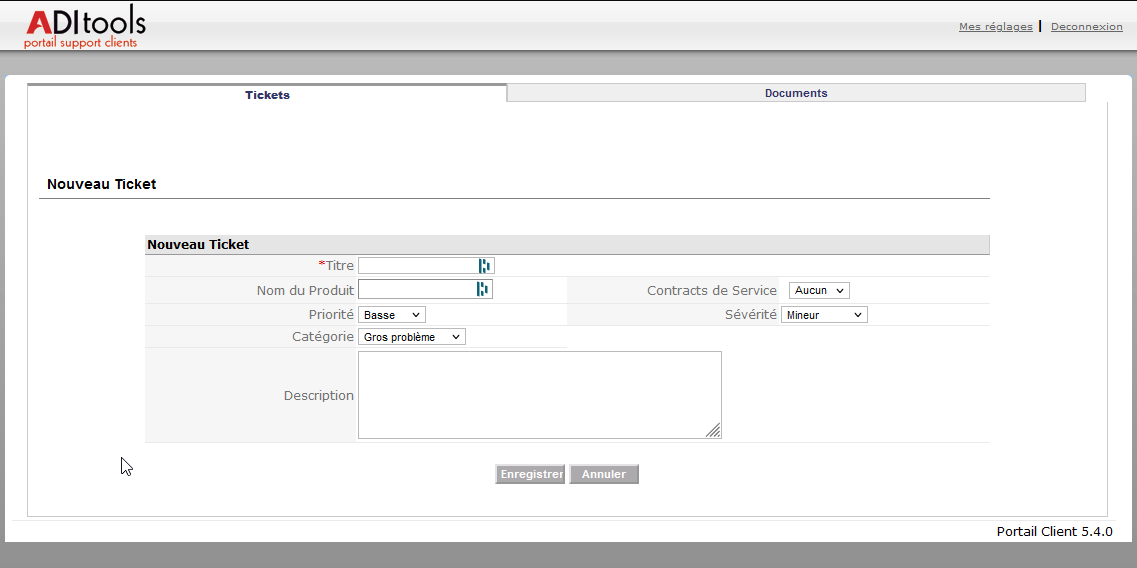
\includegraphics[width=6.3in,height=3.14722in]{image2.png}

% On peut constater que l'interface est plutôt minimaliste et
% vieillissante. Il manque certaines fonctions qui seront abordées plus
% bas.

% \textbf{Nouveau logiciel souhaité}

% Nous souhaitons migrer vers un nouveau logiciel de ticketing qui puisse
% intégrer les fonctionnalités ci-dessous~:

% Création d'incidents

% \begin{quote}
% La gestion des incidents permet de suivre et de résoudre les incidents
% signalés par les utilisateurs.
% \end{quote}

% Création de demandes de changement

% \begin{quote}
% Gestion des changements permet de planifier, suivre et gérer les
% modifications demandées par les utilisateurs.

% Exemple~: modification de ports sur le firewall, augmenter une boite aux
% lettres, etc.
% \end{quote}

% Création de tickets automatiquement

% \begin{quote}
% Cette fonctionnalité permet de planifier des interventions récurrentes
% sans les oublier. Exemple~: test de restauration
% \end{quote}

% Gestion des ressources

% \begin{quote}
% Pouvoir lié du matériel ou logiciel a un client et faire un suivi des
% modifications sur ce cette ressource.

% Exemple~: avoir le suivi des modifications comme celui qui est présent
% sur la page client du wiki.

% Intégrer du matériel lié à un fournisseur et gérer sa garantie. Exemple
% NAS ANANDA.

% Gérer les renouvellements~: des certificats

% Gérer les renouvellements~: des noms de domaines
% \end{quote}

% Inventaires

% \begin{quote}
% Lister l'ensemble des machines (connecteur OCS)
% \end{quote}

% Tableaux de bord et rapports

% Avoirs des stats et indicateurs sur ce qui nous prend le plus de temps
% dans le support.

% Ergonomique

% \begin{quote}
% Il faut que le logiciel soit intuitif et ergonomique. Que l'utilisateur
% ne soit pas rebuté par la complexité d'ouverture d'un ticket.
% \end{quote}

% Ouverture de ticket via email

% Fermeture de ticket automatique après un délai de non-réponse

% Personnalisation graphique

% \begin{quote}
% Nous souhaitons que l'application puisse se personnaliser aux couleurs
% de la société et d'y insérer le logo.
% \end{quote}

% Récupération des données ticketing vtiger

% \begin{quote}
% Seulement si cette récupération est facile. Ne pas perdre du temps sur
% cette récupération.
% \end{quote}

% Fonctions annexes

% Gestion des baies racks du datacenter

    
    % Pós Textuais
    % \nocite{*}
    % \include{pos-textuais/referencias}

\end{document}
